\documentclass[10pt, oneside]{article}
\usepackage[a4paper, total={5.5in, 9in}]{geometry}
\usepackage[ngerman]{babel}

\usepackage{blindtext}
\usepackage{titlesec}
\usepackage{amsmath}
\usepackage[hidelinks]{hyperref}
\usepackage{parskip}
\usepackage{graphicx}
\usepackage{longtable}
\usepackage[shortlabels]{enumitem}
\usepackage{multirow}
\usepackage{nccmath}
\usepackage{rotating}
\usepackage{makecell}
\usepackage{multicol}
\usepackage{capt-of}
\usepackage{csquotes}
\usepackage{amsfonts}
\usepackage{caption}

\captionsetup[table]{position=bottom}

\titleformat{\section}
    {\normalfont\Large\bfseries}{}{0pt}{}

\let\oldsection\section
\renewcommand{\section}{
  \renewcommand{\theequation}{\thesection.\arabic{equation}}
  \oldsection}
\let\oldsubsection\subsection
\renewcommand{\subsection}{
  \renewcommand{\theequation}{\thesubsection.\arabic{equation}}
  \oldsubsection}

\makeatletter
\renewcommand{\maketitle}{
    \bgroup
    \centering
    \par\LARGE\@title  \\[20pt]
    \par\large\@author \\[10pt]
    \par\large\@date
    \par
    \egroup
}
\makeatother


\title{Mathematische Grundlagen\\[5pt]\Large WiSe 2024/25\\[10pt]\Large L{\"o}sungen zu den Aufgaben 23, 28, 29 und 31}
\author{Volodymyr But}
\date{}

% - - - - - - - - - - - - - - - - - - - - - - - - - - - - - - - - - - - - - - %

\begin{document}
\sloppy

\maketitle
\vspace{25px}

\section{Aufgabe 23}

Bestimmen Sie die inverse Abbildung zu folgenden Funktionen
\begin{equation*}
    \begin{aligned}
        f_1 &: \mathbb{R} \rightarrow \mathbb{R},\ x \mapsto 10x \text{,} \\[5pt]
        f_2 &: \mathbb{R} \rightarrow \mathbb{R},\ x \mapsto \dfrac{1}{10}x \text{,} \\[5pt]
        f_3 &: X \rightarrow X,\ x \mapsto x^2 \text{,} \\[5pt]
        f_4 &: X \rightarrow X,\ x \mapsto \sqrt{x} \text{,}
    \end{aligned}
\end{equation*}
wobei $X = \{x \in \mathbb{R} : x \geq 0 \}$. Rechnen Sie dazu auch nach, dass
die Umkehrabbildungen jeweils die Bedingungen aus der Definition (der
Umkehrabbildung) erf"ullen.
\begin{equation*}
    \begin{array}{rcccl}
        f_1^{-1} &:& \mathbb{R} \rightarrow \mathbb{R},\ 10x \mapsto x &\iff& x \mapsto \dfrac{x}{10} \text{,} \\[10pt]
        f_1^{-1} &:& \mathbb{R} \rightarrow \mathbb{R},\ \dfrac{x}{10} \mapsto x &\iff& x \mapsto 10x \text{,} \\[10pt]
        f_1^{-1} &:& X \rightarrow X,\ x^2 \mapsto x &\iff& x \mapsto \sqrt{x} \text{,} \\[10pt]
        f_1^{-1} &:& X \rightarrow X,\ \sqrt{x} \mapsto x &\iff& x \mapsto x^2
    \end{array}
\end{equation*}
\begin{figure*}[h]
    \centering
    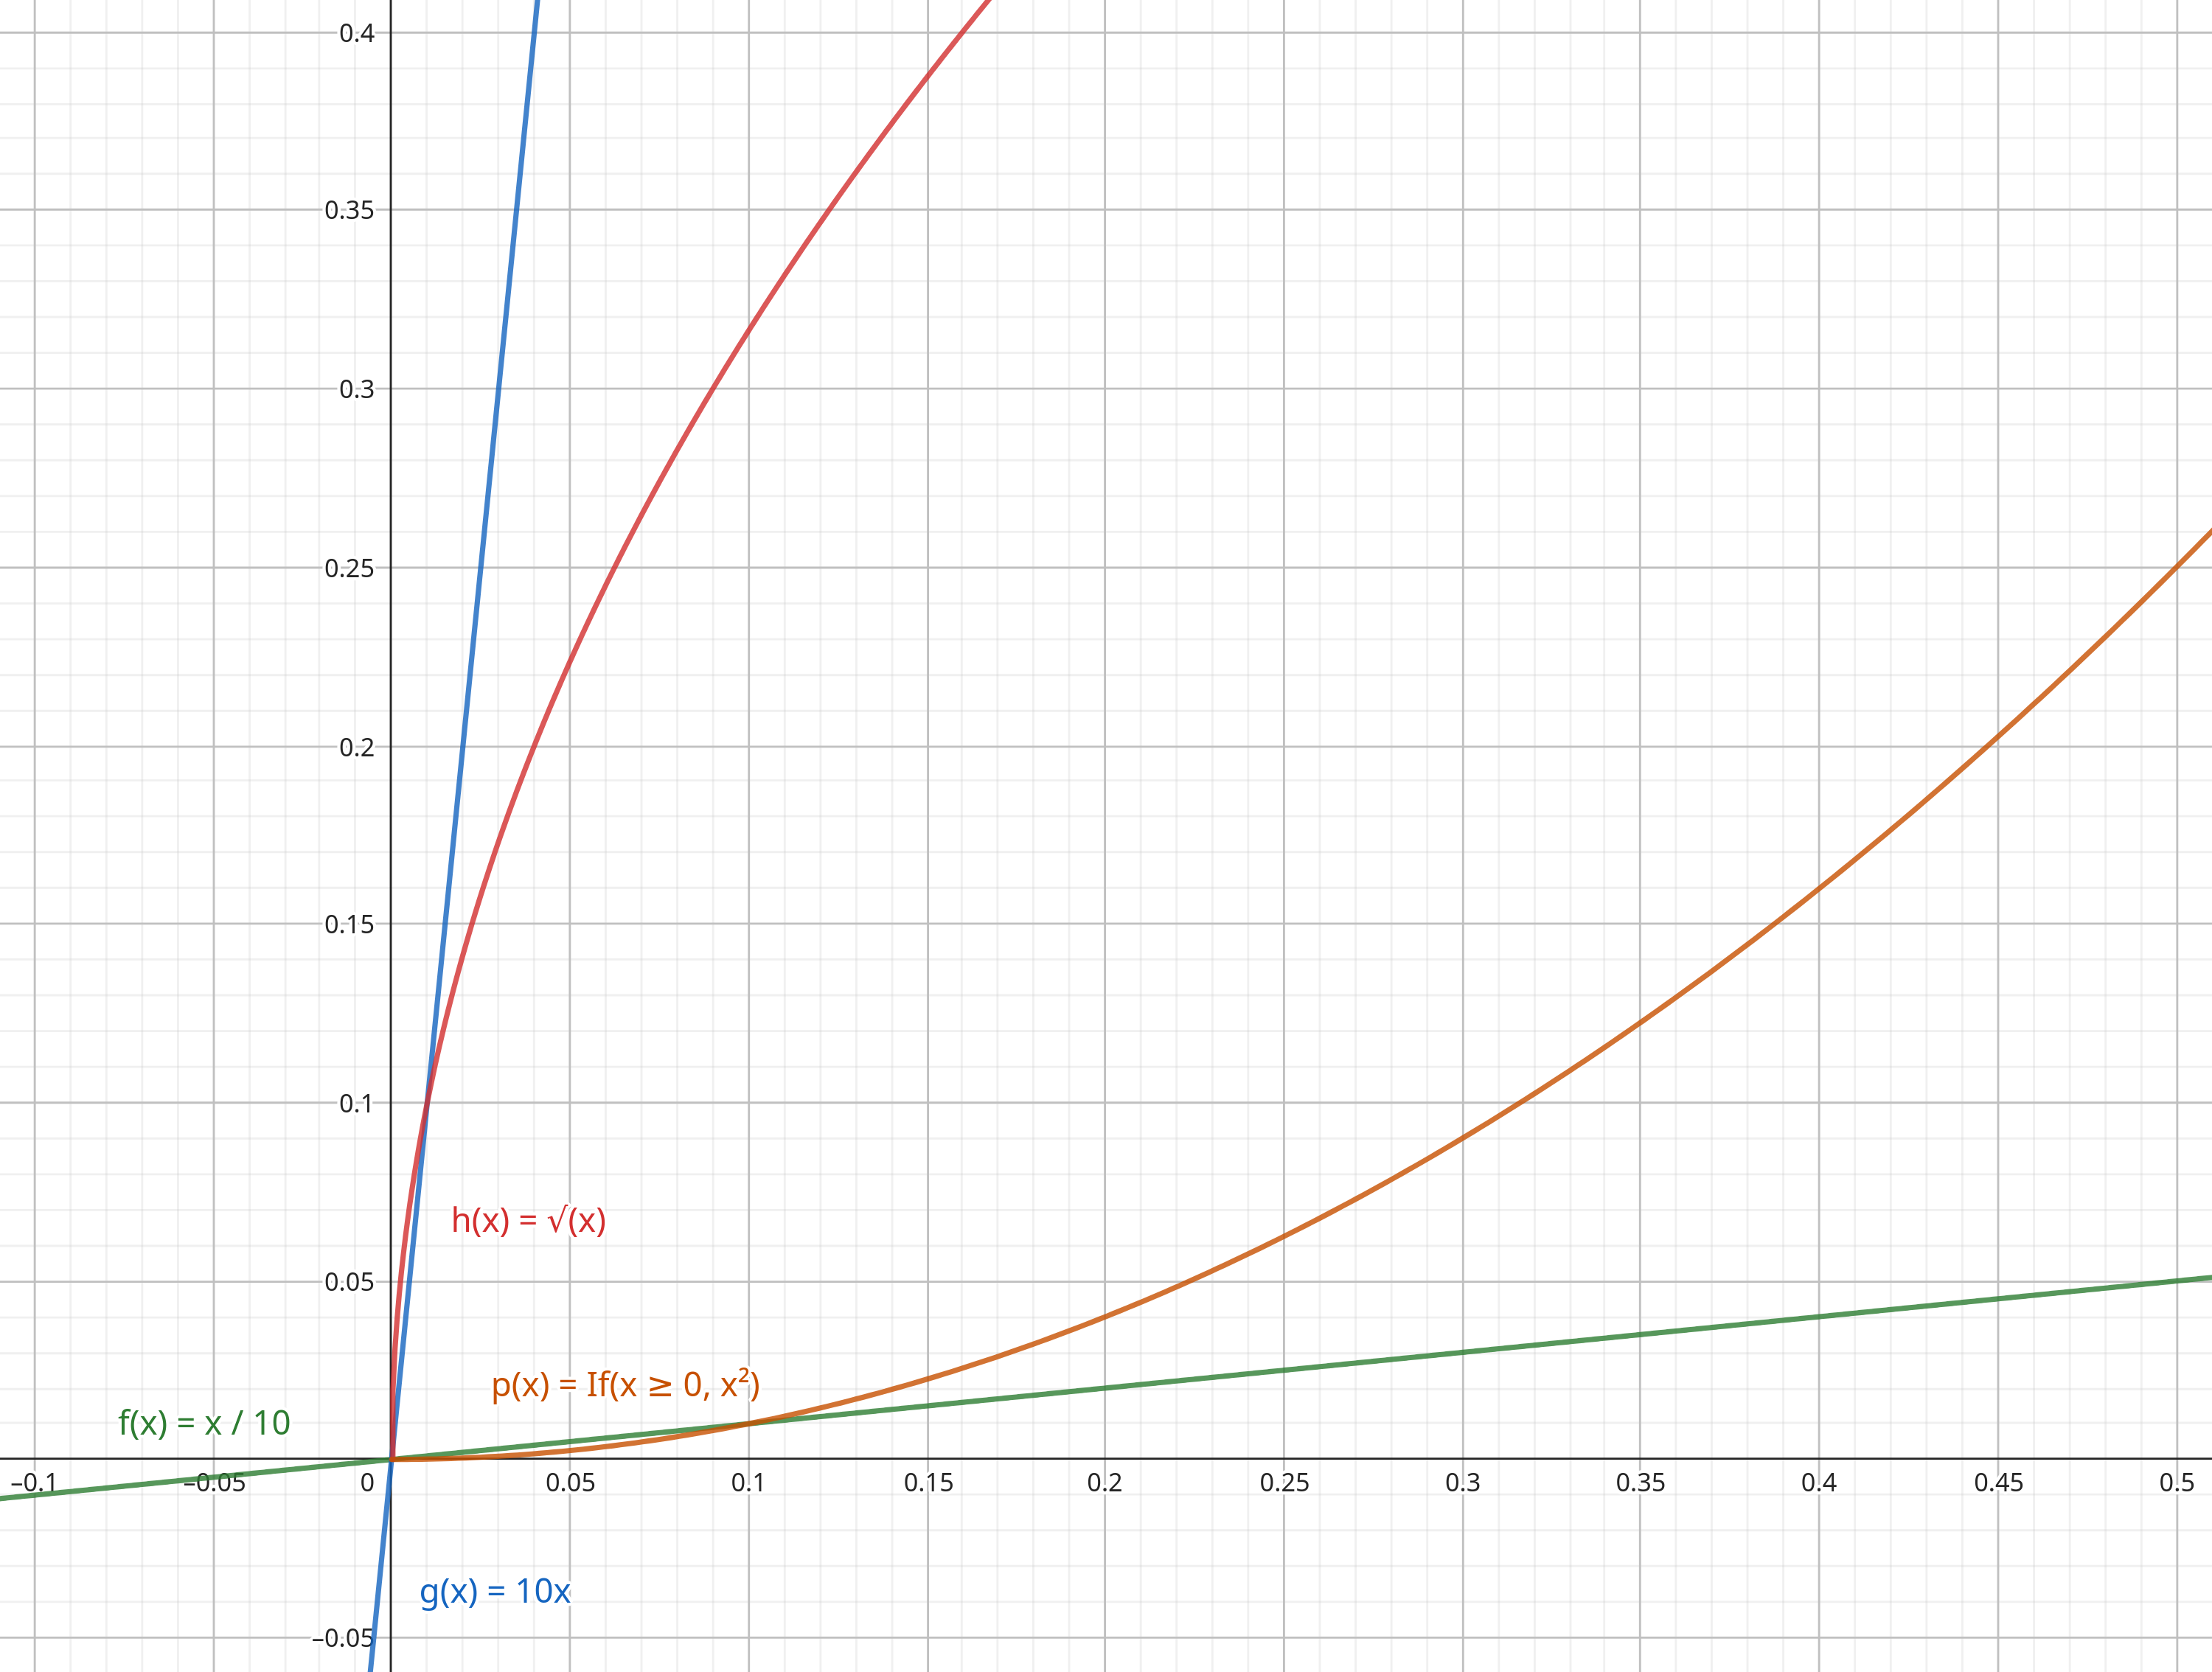
\includegraphics[width=0.7\textwidth]{./assets/23-01.png}
\end{figure*}

\section{Aufgabe 28}

Bestimmen Sie jeweils die Umkehrfunktion folgender Funktionen:
\begin{enumerate}[(a)]
    \item $f : \mathbb{R} \rightarrow \mathbb{R}$, $f(x) = x + 5$,
    \item \label{itm:28-b} $f : (0, \infty) \rightarrow (0, \infty)$, $f(x) = \dfrac{2}{x}$,
    \item \label{itm:28-c} $f : [0, \infty) \rightarrow [0, \infty)$, $f(x) = x^2 + x$.
\end{enumerate}
Rechnen Sie dazu auch nach, dass die Umkehrabbildungen jeweils die Bedingungen
aus der Definition (der Umkehrabbildung) erf"ullen. (Beachten Sie in Teil
\ref{itm:28-b} und \ref{itm:28-c} die Intervallnotation aus dem Anhang des Skripts)

\begin{enumerate}[(a)]
    \item $f^{-1} : \mathbb{R} \rightarrow \mathbb{R}$, $f^{-1}(x) = x - 5$
    \item $f^{-1} : (0, \infty) \rightarrow (0, \infty)$, $f^{-1}(x) = \dfrac{2}{x}$
    \item $f^{-1} : [0, \infty] \rightarrow [0, \infty)$, $f^{-1}(x) = -\dfrac{1}{2} + \sqrt{\dfrac{1}{4} + x}$ \\[5pt]
        \textbf{Beweis:}\\[2pt]
        \begin{equation*}
            \begin{gathered}
                \begin{aligned}[t]
                          &x = y^2 + y \\[5pt]
                    \iff\ &y^2 + y - x = 0
                \end{aligned} \\[10pt]
                \begin{array}{lcl}
                    y_{1} = - \dfrac{1}{2} + \sqrt{\left(\dfrac{1}{2}\right)^2 + x} &\quad& y_{2} = - \dfrac{1}{2} - \sqrt{\left(\dfrac{1}{2}\right)^2 + x} \\[15pt]
                    y_1   = - \dfrac{1}{2} + \sqrt{\dfrac{1}{4} + x} && y_{2} < 0 \implies \emptyset
                \end{array}
            \end{gathered}
        \end{equation*}
        \vspace{3pt}
        \begin{center}
            \underline{q.e.d.}
        \end{center}
\end{enumerate}

\pagebreak
\section{Aufgabe 29}

Es seien $M := \{1, 3, 20\}$, $N := \{-1, 4, 0\}$. Bestimmen Sie
$\mathcal{P}(M)$, $\mathcal{P}(N)$, $\mathcal{P}((M \setminus \{3\}) \times (N
\setminus \{-1\}))$.

\begin{enumerate}[(a)]
    \item $\mathcal{P}(M) = \{\emptyset, \{1\}, \{3\}, \{20\}, \{1, 3\},
                              \{1, 20\}, \{3, 20\}, \{1, 3, 20\}\}$
    \item $\mathcal{P}(N) = \{\emptyset, \{-1\}, \{4\}, \{0\}, \{-1, 4\},
                              \{-1, 0\}, \{4, 0\}, \{-1, 4, 0\}\}$
    \item $\mathcal{P}((M \setminus \{3\}) \times (N \setminus \{-1\}))$ \\[5pt]
        \textbf{Beweis:}
        \begin{equation*}
            \begin{gathered}
                (M \setminus \{3\}) = \{1, 20\} \quad\quad (N \setminus \{-1\}) = \{4, 0\} \\[5pt]
                \begin{aligned}[t]
                    (M \setminus \{3\}) \times (N \setminus \{-1\}) &= \{(x_1,
                    x_2) \in \mathbb{Z} \times \mathbb{Z} : x_1 \in (M
                    \setminus \{3\}), x_2 \in (N \setminus \{-1\})\} = \\[5pt]
                    &= \{(1, 4), (1, 0), (20, 4), (20, 0)\} \\[5pt]
                    \mathcal{P}((M \backslash\{3\}) \times(N \backslash\{-1\})) &=
                    \begin{aligned}[t]
                        \{&\emptyset,\{(1,4)\},\{(1,0)\},\{(20,4)\},\{(20,0)\},\\
                          &\{(1,4),(1,0)\},\{(1,4),(20,4)\}, \{(1,4),(20,0)\}, \\
                          &\{(1,0),(20,4)\},\{(1,0),(20,0)\},\{(20,4),(20,0)\}, \\
                          &\{(1,4),(1,0),(20,4)\},\{(1,4),(1,0),(20,0)\}, \\
                          &\{(1,4),(20,4),(20,0)\},\{(1,0),(20,4),(20,0)\}, \\
                          &\{(1,4),(1,0),(20,4),(20,0)\}\}
                    \end{aligned}
                \end{aligned} \\[5pt]
            \end{gathered}
        \end{equation*}
\end{enumerate}

\section{Aufgabe 31}

Es sei $n \in \mathbb{N}$, bestimmen Sie Formeln zur Berechnung von
\begin{equation*}
    \begin{gathered}
        |\mathcal{P}(\{\omega, f\})^n| \\
        |\mathcal{P}(\{\omega, f\}^n)|
    \end{gathered}
\end{equation*}
\begin{equation*}
    \begin{array}{rcl}
        |M^n| &=& |M|^n \\[5pt]
        |\mathcal{P}(M)| &=& 2^{|M|} \\[10pt]
        |\mathcal{P}(\{\omega, f\})^n| &=& |\mathcal{P}(\{\omega, f\})|^n = \\[5pt]
                                       &=& (2^{|\{\omega, f\}|})^n = \\[5pt]
                                       &=& (2^2)^n = \\[5pt]
                                       &=& 4^n \\[10pt]
        |\mathcal{P}(\{\omega, f\}^n)| &=& 2^{|\{\omega, f\}^n|} \\[5pt]
                                       &=& 2^{|\{\omega, f\}|^n} \\[5pt]
                                       &=& 2^{(2^n)}
    \end{array}
\end{equation*}

\end{document}
